\documentclass[twocolumn, letterpaper]{scrartcl}
\usepackage[utf8]{inputenc}
\usepackage[portuguese]{babel}
\usepackage[T1]{fontenc}
\newcommand\docID{2018-00}
\newcommand\createdOn{29 de Abril, 2019}

% Declaração de pacotes
\usepackage{padrao_logica} % template
\usepackage{float}
\usepackage{subfig}

\usepackage{xcolor}
% Definindo cores
\definecolor{beaublue}{rgb}{0.74, 0.83, 0.9}
\definecolor{softgray}{rgb}{0.9, 0.9, 0.9}

% Inicio do Documento
\begin{document}
\title{\color{triton_blue}Docker\\ \textit{Entendendo como funciona}}
% \author{Gian Lucas Cavalcante de Lima}
\date{}
\maketitle
% 
\section*{\color{triton_blue}Introdução}
Docker é uma plataforma de código aberto que roda aplicações e torna o processo de desenvolvimento e distribuição mais fácil. As aplicações que são construídas no docker são empacotados num container. Esses containers ficam rodando de forma isolada sobre o kernel do sistema operacional da máquina.\\
Apesar do sucesso recente do docker, as tecnologias de container já existem a mais de 10 anos, porém só com o docker que essa ferramenta se popularizou. O docker tornou os containers fáceis, práticos e acessíveis. Com o seu surgimento ele trouxe inovações para a tecnologia que já existia, entre suas novas capacidades, estão: facilidade para criar e controlar containers, leveza no empacotamento de container, as aplicações virtualizadas podem ser rodadas em qualquer lugar sem a necessidade de alterações. e para completar tudo, o Docker pode facilmente ser integrado com instrumentos de terceiros que ajudam na implementação e gerenciamento de containers docker.
%Esse documento é uma análise e estudo sobre as funcionalidades do Docker, com o objetivo de entender para que funciona cada ferramenta que constitui o Docker como um todo.

\section*{\color{triton_blue}O que é um Container?}
Containers não são máquinas virtuais (VMs), mas eles tem o mesmo objetivo de uma VM, isolar uma aplicação e suas dependências numa unidade auto-contida que pode ser rodada em qualquer lugar. A principal diferença entre eles esta na sua arquitetura.\\
Uma VM é essencialmente uma emulação de um computador real que executa programas como um computador real. Elas rodam em cima de uma máquina física usando uma camada extra chamada \textit{hypervisor}, como pode ser observado na Figura \ref{fig:hypervisor_layer}.\\
Como a VM tem seu próprio sistema operacional virtual, o \textit{hypervisor} tem como papel principal prover a VM com uma plataforma aonde ela possa gerenciar e executar seu sistema operacional guest. Isso permite que a máquina host possa compartilhar seus recursos entre as máquinas virtuais que estão rodando como guests em cima dela.

\paragraph{Hypervisor:} é um pedaço de software, firmware, ou hardware em que a VM roda em cima. O \textit{hypervisor} por si só roda na máquina física, que é chamada de \textit{máquina host}. O host provê os recursos para as máquinas virtuais, incluindo RAM e CPU. Esses recursos são divididos entre as VMs e pode ser distribuído como for necessário.\\

\noindent Diferente das VMs que provem a virtualização completa de hardware de um sistema operacional Guest rodando por cima do sistema operacional do Host, os containers fazem uma abordagem diferente, ele provê uma virtualização à nível do sistema operacional, para isso ele usa de alguns recursos do sistema para abstrair o \textit{user space}.\\
Para todas as intenções e propósitos, containers são parecidos com VMs. Por exemplo, eles tem espaço privado de processamento, podem executar comandos como \textit{root}, tem interface de rede privada e endereços de IP, podem montar sistemas de arquivos, e etc. A grande diferença dos containers para máquinas virtuais são que eles compartilham o kernel da máquina host.\\ 
Containers tem empacotado somente o \textit{user space}, e não o kernel ou hardware virtual como numa VM. Cada container possui isolado somente suas informações próprias e dependências, enquanto que toda a arquitetura do sistema operacional é compartilhada entre os containers, como pode ser visto na Figura \ref{fig:docker_layer} as únicas partes que são criadas do zero são os \textit{bins} e \textit{libs}. Isso que torna os containers tão leves.

\begin{figure}[!tbp]
\centering
    \subfloat[Camadas VM]{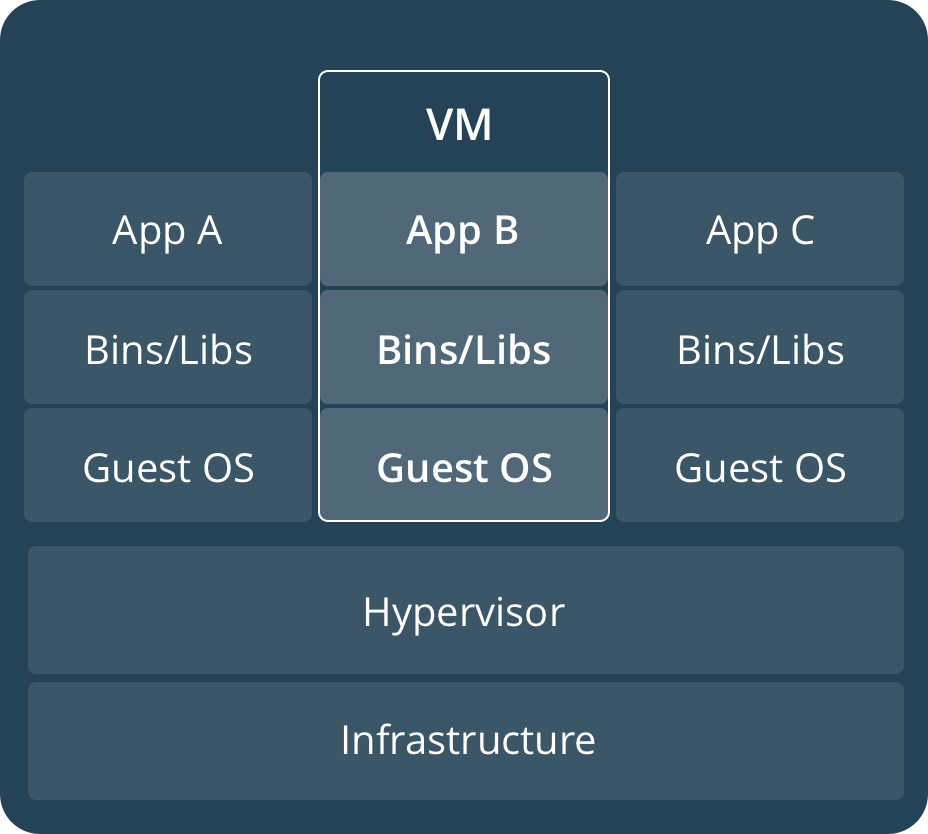
\includegraphics[width=0.24\textwidth]{imgs/camadas_vm.png}\label{fig:hypervisor_layer}}
    \hfill
    \subfloat[Camadas Container]{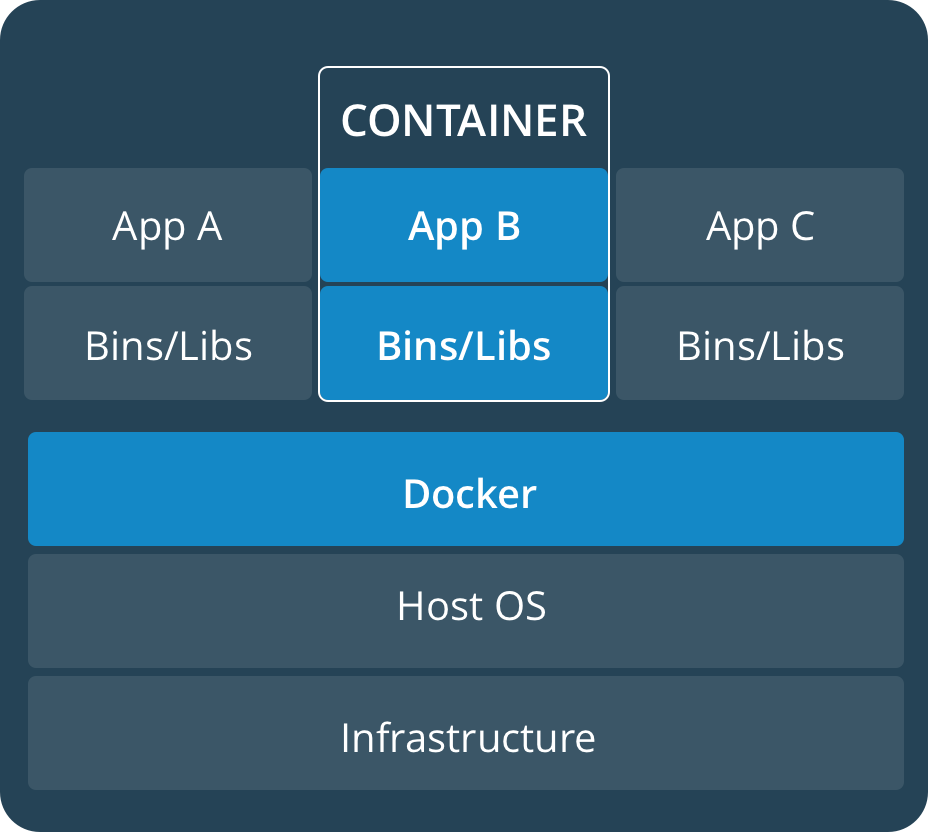
\includegraphics[width=0.24\textwidth]{imgs/camadas_container.png}\label{fig:docker_layer}}
    \caption{Comparativo camadas de VMs vs. Containers}
\end{figure}

\subsection*{\color{triton_blue}User Space}
Essencialmente o \textit{User Space} é formado pelo \textit{Namespaces} e \textit{CGroups}, além disso o Docker também faz uso de drivers de armazenamento como AUFS, DeviceMapper, Overlay BTRFS, e VFS.
\paragraph{Namespaces} provê os containers com sua própria visão do sistema Linux subjacente a ele, limitando o que o container pode ver e acessar. Quando você roda um container, o Docker cria namespaces que o container em específico irá utilizar. Existem vários namespaces no kernel dos quais o Docker faz uso, por exemplo:
\begin{itemize}
    \item \textsc{\textbf{net:}} provê ao container sua própria visão da rede, com isso ele possui seus próprios dispositivos de rede, endereços de IP, tabelas de roteamento de IP, numeros de portas, etc.
    \item \textsc{\textbf{pid:}} provê ao container seu próprio escopo de processos do sistema, dando inclusive numeração própria para os processos dentro do container.
    \item \textsc{\textbf{mount:}} dá ao container sua visão de volumes montandos no sistema.
    \item \textsc{\textbf{uts:}} padrão para UNIX Timesharing System. O UTS permite que o container tenha seu próprio \textit{hostname} e \textit{NIS domain name}.
    \item \textsc{\textbf{ipc:}} padrão para InterProcess Communication. IPC é responsável por isolar os recursos IPC entre os processos rodando dentro de cada container.
    \item \textsc{\textbf{user:}} esse namespace é usado para isolar os usuários dentro de cada container. Ele funciona permitindo que containers tenham diferentes visões dos userID e groupID se comparado com o sistema host. Como resultado, o userID e groupID de um processo pode ser diferente dentro e fora de um usuário no namespace, isso também permite que um processo tenha usuário sem privilégios fora de um container sem sacrificar o privilégio de root dentro do mesmo.
\end{itemize}
\paragraph{CGroups} ou Control Groups é uma característica do kernel Linux que isola, prioriza, e toma conta do uso de recursos (CPU, Memória, Leitura e Escrita do Disco, Rede, etc.) de um conjunto de processos. Nesse sentido, o CGroups certifica que o Docker use somente os recursos que ele necessita. CGroups também garante que um único container não exaura um de seus recursos e leve todo o sistema a cair.

\section*{\color{triton_blue}O que é Docker?}
Como dito na introdução, Docker é um projeto de código aberto baseado no Linux Containers (LXC). E para que ele funcione o Docker utiliza alguns dos recursos do kernel Linux como o \textit{Namespaces} e \textit{CGroups} para criar containers sobre o sistema operacional.\\
Porém sabendo que o Docker Container não são os pioneiros na tecnologia de containers, o que tornou ele tão popular foram quatro virtudes que ele possui.
\begin{enumerate}
    \item \textbf{Fácil de usar:} Docker foi criado de forma a ser muito mais fácil, tendo em vista que desenvolvedores, administradores de sistemas, arquitetos e outros usuários possam tomar vantagem de containers para rapidamente construir e testar aplicações. Ele permite que qualquer um possa empacotar uma aplicação no seu computador pessoal e possa move-lo para outra plataforma, seja ela uma rede privada, nuvem pública ou qualquer outro local e possa rodá-lo sem precisar de modificação.
    \item \textbf{Velocidade:} Docker Containers são muito leves e rápidos. Como eles compartilham do kernel do host, eles precisam de muito poucos recursos para funcionar. É póssivel criar uma container em questão se segundos e já começar a utilizar.
    \item \textbf{Modularidade e Escalabilidade:} Docker torna fácil a divisão das funcionalidades da sua aplicação em containers individuais. Por exemplo você pode ter seu banco de dados rodando num container, sua aplicação noutro, e os volumes num terceiro. E facilmente interligar todas elas para criar a aplicação completa.
    \item \textbf{Docker Hub:} E por último, mas não menos importante. O Docker Hub, nele os usuários e até mesmo as grandes empresas disponibilizam imagens prontas para uso aonde todos os usuários tem acesso e podem usufruir de um grande acervo de imagens para utilizar em seus projetos.
\end{enumerate}
\subsection*{\color{triton_blue}Camadas}
O Docker funciona baseado em camadas, essas camadas são imagens que contem pedaços do sistema e são imutáveis (como pode ser observado na Figura \ref{fig:docker_layers}). Ao criar uma imagem de um container, o Docker compila cada parte do sistema numa camada e cria uma subimagem com aquele pedaço do sistema. Dessa forma ele consegue reaproveitar essas subimagens para a criação de uma nova imagem que tenha pedaços em comum com outro já existente, isso torna o Docker muito mais leve e de fácil escalonação.\\
Uma imagem é formada pelo empilhamento de várias camadas, mas essas camadas são somente de leitura e no topo de tudo a ultima camada é a única camada que pode ser escrita, então ao modificar um arquivo de uma cada anterior o sistema cria uma cópia daquele arquivo na camada superior e escreve nele.

\begin{figure}
    \centering
    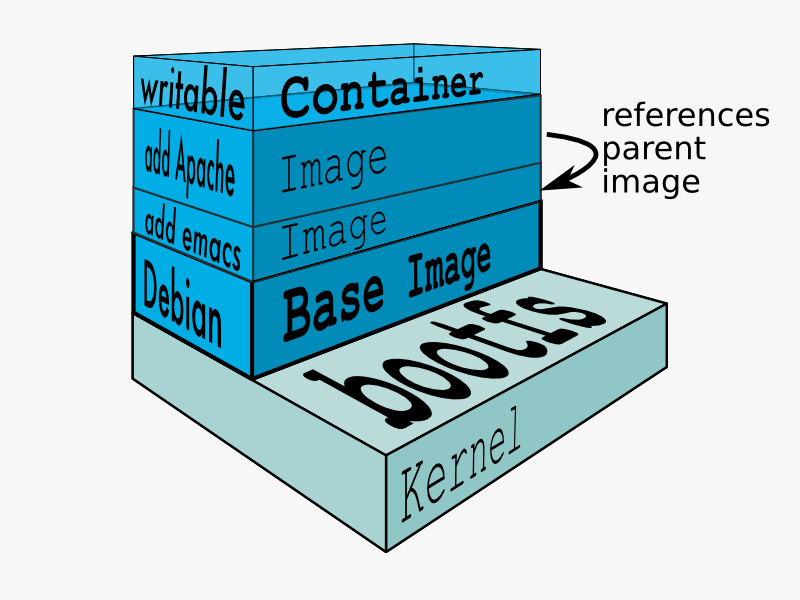
\includegraphics[scale=0.25]{imgs/docker_layers.png}
    \caption{Camadas de uma Imagem}
    \label{fig:docker_layers}
\end{figure}

\section*{\color{triton_blue}Gerenciadores}
O Docker é dividido em vários gerenciadores, cada gerenciador é responsável por controlar uma das partes do programa como um todo. Sendo assim se você quer por exemplo parar um container usa-se.
\begin{center}
    \texttt{\$ docker container stop \textit{"nome\_do\_container"}}
\end{center}
Ou para parar um serviço usa-se.
\begin{center}
    \texttt{\$ docker service stop \textit{"nome\_do\_serviço"}}
\end{center}
Ou mesmo se quiser saber que portas estão abertas num container.
\begin{center}
    \texttt{\$ docker port \textit{"nome\_do\_container"}}
\end{center}
Dessa forma é muito fácil e intuitivo usar o Docker e gerir o ambiente. A seguir veremos uma breve explicação sobre alguns dos gerenciadores mais importantes e quais os seus comandos.

\subsection*{\color{triton_blue}container}
O \texttt{container} é responsável por gerir os containers existentes, com ele se fará todas as ações à respeito dos containers, como criar, iniciar, parar, deletar, e etc.\\
\indent\fcolorbox{lightgray}{softgray}{%
    \minipage[t]{0.9\linewidth}%
    \centering\vspace{2px}
        \textsc{comandos:}\\
        \textbf{attach, commit, cp, create, diff, exec, export, inspect, kill, logs, ls, pause, port, prune, rename, restart, rm, run, start, stats, stop, top, unpause, update, wait}
    \endminipage%
}
\subsection*{\color{triton_blue}image}
O \texttt{image} é responsável pelas imagens, desde a criação de imagens como pela gestão das imagens já existentes na máquina. Com ele além de poder criar imagens, também pode-se baixar e subir imagens para um registry privado ou público como Docker Hub.\\
\indent\fcolorbox{lightgray}{softgray}{%
    \minipage[t]{0.9\linewidth}%
    \centering\vspace{2px}
        \textsc{comandos:}\\
        \textbf{build, history, import, inspect, load, ls, prune, pull, push, rm, save, tag}
    \endminipage%
}
\subsection*{\color{triton_blue}service}
O \texttt{service} é responsável pelos serviços. Caso seja necessário escalar seus serviços é por meio desse gerenciador que se faz.\\
\indent\fcolorbox{lightgray}{softgray}{%
    \minipage[t]{0.9\linewidth}%
    \centering\vspace{2px}
        \textsc{comandos:}\\
        \textbf{create, inspect, logs, ls, ps, rm, rollback, scale, update}
    \endminipage%
}
\subsection*{\color{triton_blue}swarm}
O \texttt{swarm} é responsável pela gestão dos swarms, como criar uma orquestração, adicionar e remover máquinas ao cluster.\\
\indent\fcolorbox{lightgray}{softgray}{%
    \minipage[t]{0.9\linewidth}%
    \centering\vspace{2px}
        \textsc{comandos:}\\
        \textbf{ca, init, join, join-token, leave, unlock, unlock-key, update}
    \endminipage%
}
\vspace{20px}\\
Além dessas também existem as \texttt{builder}, \texttt{config}, \texttt{engine}, \texttt{network}, \texttt{node}, \texttt{plugin}, \texttt{secret}, \texttt{stack}, \texttt{system}, \texttt{trust} e \texttt{volume}. Para mais informações sobre quais os comandos de cada gerenciador e parâmetros é possível acessar os manuais do docker usando o parâmetro \textit{"--help"} na chamada dos comandos, por exemplo, para ver comandos de um gerenciador.
\begin{center}
    \texttt{\$ docker \textit{"serviço"} --help}
\end{center}
Ou para saber sobre um comando em específico.
\begin{center}
    \texttt{\$ docker \textit{"serviço"} \textit{"comando"} --help}
\end{center}
\section*{\color{triton_blue}Dockerfile}
O Dockerfile é um arquivo de texto simples com instruções de construção de imagem, seria algo como a \textit{blueprint} de uma imagem, aonde são descritos todas as características de uma imagem. Nele é possível definir desde a imagem de base para a construção para a nova, quanto quais portas estarão abertas, qual aplicação estará rodando dentro dela, etc.\\
Para isso dentro do arquivo são escritos algumas linhas de instruções iniciadas com palavras-chaves que o Docker reconhece e interpreta o que esta escrito. Após escrever o Dockefile basta rodar \texttt{\$ docker image build \textit{"caminho\_para\_Dockerfile"}} para construir a imagem.\\
\indent\fcolorbox{lightgray}{softgray}{%
    \minipage[t]{0.9\linewidth}%
    \centering\vspace{2px}
        \textsc{palavras-chaves:}\\
        \textbf{\textsc{from, run, cmd, label, expose, env, add, copy, entrypoint, volume, user, workdir, arg, onbuild, stopsignal, healthcheck, shell}}
    \endminipage%
}

\section*{\color{triton_blue}Docker Compose \& Docker Stack}
O Docker Compose é uma ferramenta extra ao Docker criada para tornar o gerenciamento de vários containers de uma aplicação mais dinâmico. Nascido como um projeto paralelo ao Docker em si, diferente do Docker que é escrito em Go, o Docker Compose foi escrito em Python. Com ele é possível subir vários containers de uma só vez e definir todo seu comportamento de operação.\\
Tudo começa com a criação de um arquivo chamado Composefile com extensão YAML aonde se é descrito cada um dos serviços da aplicação, junto de suas conexões, volumes, políticas de funcionamento, dependências entre serviços, ação na queda de um container, e muito mais. A ideia do Docker Compose é tornar o processo de subir aplicações muito mais rápido e fácil, dispensando a necessidade de se subir cada serviço manualmente, além de se evitar erros por ter que digitar comandos enormes.\\
Além do Docker Compose mais recentemente foi o \texttt{docker stack} que foi desenvolvido com objetivo similar ao do Compose. As principais diferenças entre eles são que o Docker Stack é uma ferramenta dentro do próprio Docker e foi escrito em Go, isso foi feito para centralizar as ferramentas do Docker e simplificar seu desenvolvimento. Além disso o Docker Stack faz parte do modo Swarm do Docker e não consegue ele mesmo construir uma imagem como o Compose faz (o Docker Stack espera que todas as imagens a serem usadas já estejam construídas).\\
No Funcionamento Docker Stack foi pensado para tornar simples o intercâmbio com o Docker Compose, ambos aceitam o mesmo arquivo de configuração YAML (o Docker Stack aceita Composefile de versão 3 acima), com exceção que o Stack não reconhece alguns parâmetros que o Compose reconhece e vice-versa, mas ambos foram configurados para reconhecer e ignorar esses comandos diferentes. No mais, o Docker Stack faz tudo que o Docker Compose faz.


\bibliographystyle{unsrtnat}
% \bibliography{biblio}
% \begin{thebibliography}{9}
% \end{thebibliography}
% \blurb
\end{document}
